\Cref{no_water_table,water_table,solution1_table,solution2_table,solution3_table,solution4_table} provide the raw data for polarization angle, intesnity, and intensity error. The error in each polarization measurement was $\pm 2$ degress, while the error in intensity measurement varied.

\begin{table}[H]
	\begin{center}
		\resizebox{\columnwidth}{!}{%
		\begin{tabular}{ccc}
			\toprule
			Polarization $\pm 2$ (degrees) & Intensity (arb. units) & Intensity $\pm$ (arb. units) \\
			\midrule
			\hline
			& No Beaker & \\
			\hline
			90 & 0.00 & 0.01 \\
			80 & 0.14 & 0.01 \\
			70 & 0.47 & 0.01 \\
			60 & 1.00 & 0.03 \\
			50 & 1.65 & 0.03 \\
			40 & 2.40 & 0.03 \\
			30 & 3.0 & 0.1 \\
			20 & 3.4 & 0.1 \\
			10 & 3.6 & 0.1 \\
			0 & 3.8 & 0.1 \\
			\hline
			& Small Beaker & \\
			\hline
			90 & 0.00 & 0.01 \\
			80 & 0.05 & 0.01 \\
			70 & 0.40 & 0.01 \\
			60 & 0.78 & 0.01 \\
			50 & 1.25 & 0.03 \\
			40 & 1.75 & 0.03 \\
			30 & 2.20 & 0.03 \\
			20 & 2.55 & 0.03 \\
			10 & 2.70 & 0.03 \\
			0 & 2.85 & 0.03 \\
			\hline
			& Medium Beaker & \\
			\hline
			90 & 0.00 & 0.01 \\
			80 & 0.12 & 0.01 \\
			70 & 0.47 & 0.01 \\
			60 & 0.94 & 0.01 \\
			50 & 1.50 & 0.03 \\
			40 & 2.10 & 0.03 \\
			30 & 2.65 & 0.03 \\
			20 & 3.0 & 0.1 \\
			10 & 3.2 & 0.1 \\
			0 & 3.3 & 0.1 \\
			\hline
			& Large Beaker & \\
			\hline
			90 & 0.00 & 0.01 \\
			80 & 0.10 & 0.01 \\
			70 & 0.37 & 0.01 \\
			60 & 0.80 & 0.01 \\
			50 & 1.30 & 0.03 \\
			40 & 1.80 & 0.03 \\
			30 & 2.25 & 0.03 \\
			20 & 2.50 & 0.03 \\
			10 & 2.80 & 0.03 \\
			0 & 2.90 & 0.03 \\
			\bottomrule
		\end{tabular}}
	\end{center}
	\caption{Data for the no beaker, small beaker, medium beaker, and large beaker without water. The polarization was measured in degrees, and both intensity and intensity error were measured in arbitrary units.}
	\label{no_water_table}
\end{table}

Figures 2-7 show the intensity versus polarization with each separate graph containing data from a single solution. Each graph demonstrates the curves for different beaker sizes (small, medium, large) as seen by the legend.

\begin{figure}[H]
    \begin{center}
        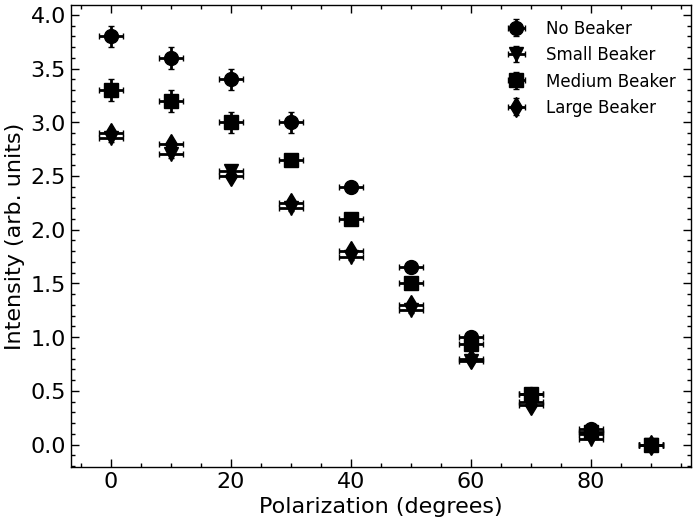
\includegraphics[width=\columnwidth]{../figures/no_water.png}
    \end{center}
    \caption{Intensity vs. Polarization for varying beaker sizes with no water. The polarization was measured in degrees and the intensity was measured in arbitrary units.}
    \label{no_water_figure}
\end{figure}

\begin{table}[H]
	\begin{center}
		\resizebox{\columnwidth}{!}{%
		\begin{tabular}{ccc}
			\toprule
			Polarization $\pm 2$ (degrees) & Intensity (arb. units) & Intensity $\pm$ (arb. units) \\
			\midrule
			\hline
			& Small Beaker & \\
			\hline
			90 & 0.88 & 0.01 \\
			80 & 2.65 & 0.01 \\
			70 & 6.20 & 0.03 \\
			60 & 12.00 & 0.03 \\
			50 & 18.0 & 0.1 \\
			40 & 25.5 & 0.1 \\
			30 & 31.0 & 0.1 \\
			20 & 35.0 & 0.1 \\
			10 & 38.0 & 0.1 \\
			\hline
			& Medium Beaker & \\
			\hline
			0 & 39.00 & 0.01 \\
			90 & 0.27 & 0.01 \\
			80 & 0.88 & 0.01 \\
			70 & 2.50 & 0.03 \\
			60 & 4.60 & 0.1 \\
			50 & 7.40 & 0.1 \\
			40 & 10.0 & 0.3 \\
			30 & 12.5 & 0.3 \\
			20 & 14.5 & 0.3 \\
			10 & 15.5 & 0.3 \\
			0 & 16.0 & 0.3 \\
			\hline
			& Large Beaker & \\
			\hline
			90 & 0.09 & 0.01 \\
			80 & 0.43 & 0.01 \\
			70 & 1.30 & 0.03 \\
			60 & 2.40 & 0.03 \\
			50 & 3.9 & 0.1 \\
			40 & 5.2 & 0.1 \\
			30 & 6.6 & 0.1 \\
			20 & 7.6 & 0.1 \\
			10 & 8.2 & 0.1 \\
			0 & 8.6 & 0.1 \\
			\bottomrule
		\end{tabular}}
	\end{center}
	\caption{Data for the small beaker, medium beaker, and large beaker with water. The polarization was measured in degrees, and both intensity and intensity error were measured in arbitrary units.}
	\label{water_table}
\end{table}

\begin{figure}[H]
    \begin{center}
        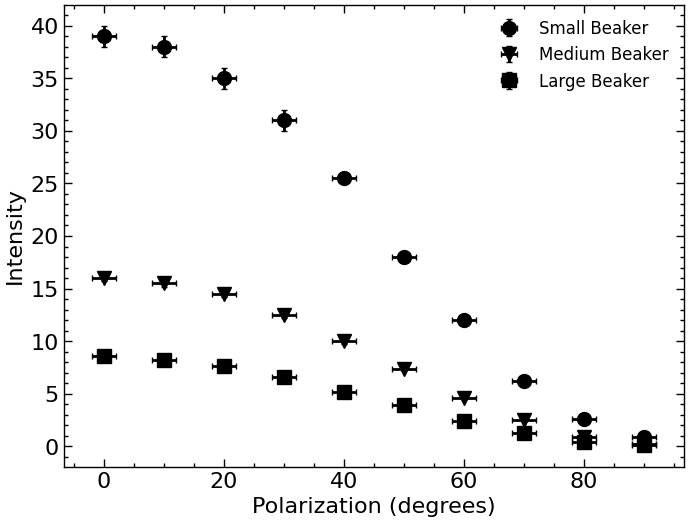
\includegraphics[width=\columnwidth]{../figures/water.png}
    \end{center}
    \caption{Intensity vs. Polarization for varying beaker sizes with water. The polarization was measured in degrees and the intensity was measured in arbitrary units.}
    \label{water_figure}
\end{figure}

\begin{table}[H]
	\begin{center}
		\resizebox{\columnwidth}{!}{%
		\begin{tabular}{ccc}
			\toprule
			Polarization $\pm 2$ (degrees) & Intensity (arb. units) & Intensity $\pm$ (arb. units) \\
			\midrule
			\hline
			& Small Beaker & \\
			\hline
			100 & 0.80 & 0.03 \\
			90 & 2.25 & 0.03 \\
			80 & 5.0 & 0.1 \\
			70 & 8.9 & 0.1 \\
			60 & 13.0 & 0.3 \\
			50 & 16.5 & 0.3 \\
			40 & 21.5 & 0.3 \\
			30 & 24.0 & 0.3 \\
			20 & 26.0 & 0.3 \\
			10 & 25.5 & 0.3 \\
			0 & 24.0 & 0.3 \\
			\hline
			& Medium Beaker & \\
			\hline
			90 & 1.90 & 0.03 \\
			80 & 3.9 & 0.1 \\
			70 & 6.2 & 0.1 \\
			60 & 9.2 & 0.1 \\
			50 & 11.5 & 0.3 \\
			40 & 13.5 & 0.3 \\
			30 & 15.0 & 0.3 \\
			20 & 15.0 & 0.3 \\
			10 & 14.5 & 0.3 \\
			0 & 13.5 & 0.3 \\
			\hline
			& Large Beaker & \\
			\hline
			90 & 1.30 & 0.03 \\
			80 & 2.50 & 0.03 \\
			70 & 4.0 & 0.1 \\
			60 & 5.4 & 0.1 \\
			50 & 6.7 & 0.1 \\
			40 & 7.6 & 0.1 \\
			30 & 8.3 & 0.1 \\
			20 & 8.5 & 0.1 \\
			10 & 8.1 & 0.1 \\
			0 & 7.2 & 0.1 \\
			\bottomrule
		\end{tabular}}
	\end{center}
	\caption{Data for the small beaker, medium beaker, and large beaker with solution 1. The polarization was measured in degrees, and both intensity and intensity error were measured in arbitrary units.}
	\label{solution1_table}
\end{table}

\begin{figure}[H]
    \begin{center}
        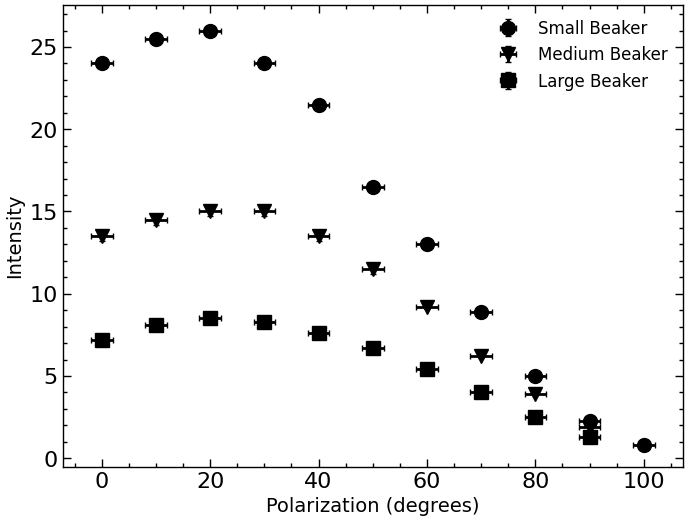
\includegraphics[width=\columnwidth]{../figures/solution1.png}
    \end{center}
    \caption{Intensity vs. Polarization for varying beaker sizes with solution 1. The polarization was measured in degrees and was intensity is measured in arbitrary units.}
    \label{solution1_figure}
\end{figure}

\begin{table}[H]
	\begin{center}
		\resizebox{\columnwidth}{!}{%		
		\begin{tabular}{ccc}
			\toprule
			Polarization $\pm 2$ (degrees) & Intensity (arb. units) & Intensity $\pm$ (arb. units) \\
			\midrule
			\hline
			& Small Beaker & \\
			\hline
			90 & 5.0 & 0.1 \\
			80 & 7.7 & 0.1 \\
			70 & 11.0 & 0.3 \\
			60 & 14.0 & 0.3 \\
			50 & 17.0 & 0.3 \\
			40 & 18.5 & 0.3 \\
			30 & 19.0 & 0.3 \\
			20 & 19.5 & 0.3 \\
			10 & 17.5 & 0.3 \\
			0 & 13.5 & 0.3 \\
			\hline
			& Medium Beaker & \\
			\hline
			90 & 9.4 & 0.1 \\
			80 & 13.5 & 0.3 \\
			70 & 17.5 & 0.3 \\
			60 & 21.0 & 0.3 \\
			50 & 23.0 & 0.3 \\
			40 & 23.5 & 0.3 \\
			30 & 24.5 & 0.3 \\
			20 & 22.0 & 0.3 \\
			10 & 19.5 & 0.3 \\
			0 & 15.5 & 0.3 \\
			\hline
			& Large Beaker & \\
			\hline
			90 & 2.2 & 0.03 \\
			80 & 3.1 & 0.1 \\
			70 & 4.3 & 0.1 \\
			60 & 5.2 & 0.1 \\
			50 & 5.8 & 0.1 \\
			40 & 5.9 & 0.1 \\
			30 & 6.4 & 0.1 \\
			20 & 5.8 & 0.1 \\
			10 & 5.1 & 0.1 \\
			0 & 3.7 & 0.1 \\
			\bottomrule
		\end{tabular}}
	\end{center}
	\caption{Data for the small beaker, medium beaker, and large beaker with solution 2. The polarization was measured in degrees, and both intensity and intensity error were measured in arbitrary units.}
	\label{solution2_table}
\end{table}

\begin{figure}[H]
    \begin{center}
        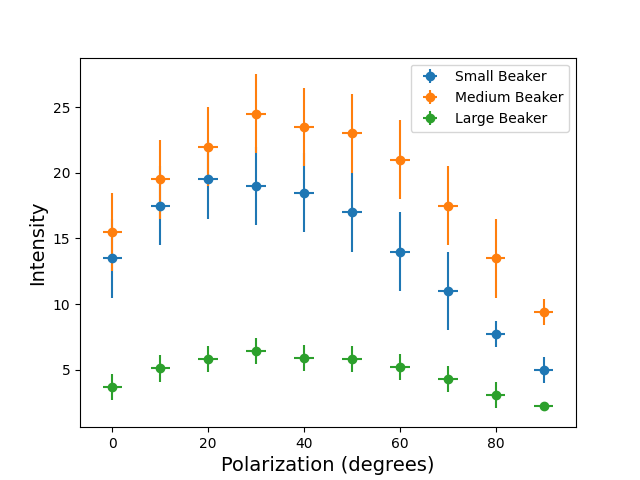
\includegraphics[width=\columnwidth]{../figures/solution2.png}
    \end{center}
    \caption{Intensity vs. Polarization for varying beaker sizes with solution 2. The polarization was measured in degrees and the intensity was measured in arbitrary units.}
    \label{solution2_figure}
\end{figure}

\begin{table}[H]
	\begin{center}
		\resizebox{\columnwidth}{!}{%
		\begin{tabular}{ccc}
			\toprule
			Polarization $\pm 2$ (degrees) & Intensity (arb. units) & Intensity $\pm$ (arb. units) \\
			\midrule
			\hline
			& Small Beaker & \\
			\hline
			90 & 1.7 & 0.03 \\
			80 & 5.3 & 0.1 \\
			70 & 11.0 & 0.3 \\
			60 & 17.5 & 0.3 \\
			50 & 26.0 & 0.3 \\
			40 & 34 & 1 \\
			30 & 40 & 1 \\
			20 & 44 & 1 \\
			10 & 46 & 1 \\
			0 & 46 & 1 \\
			\hline
			& Medium Beaker & \\
			\hline
			90 & 0.58 & 0.01 \\
			80 & 1.75 & 0.03 \\
			70 & 3.4 & 0.1 \\
			60 & 5.8 & 0.1 \\
			50 & 8.4 & 0.1 \\
			40 & 11.0 & 0.3 \\
			30 & 12.0 & 0.3 \\
			20 & 13.0 & 0.3 \\
			10 & 13.5 & 0.3 \\
			0 & 13.5 & 0.3 \\
			\hline
			& Large Beaker & \\
			\hline
			90 & 0.41 & 0.01 \\
			80 & 1.10 & 0.03 \\
			70 & 2.25 & 0.03 \\
			60 & 3.6 & 0.1 \\
			50 & 5.1 & 0.1 \\
			40 & 6.4 & 0.1 \\
			30 & 7.3 & 0.1 \\
			20 & 8.0 & 0.1 \\
			10 & 8.2 & 0.1 \\
			0 & 8.0 & 0.1 \\
			\bottomrule
		\end{tabular}}
	\end{center}
	\caption{Data for the small beaker, medium beaker, and large beaker with solution 3. The polarization was measured in degrees, and both intensity and intensity error were measured in arbitrary units.}
	\label{solution3_table}
\end{table}

\begin{figure}[H]
    \begin{center}
        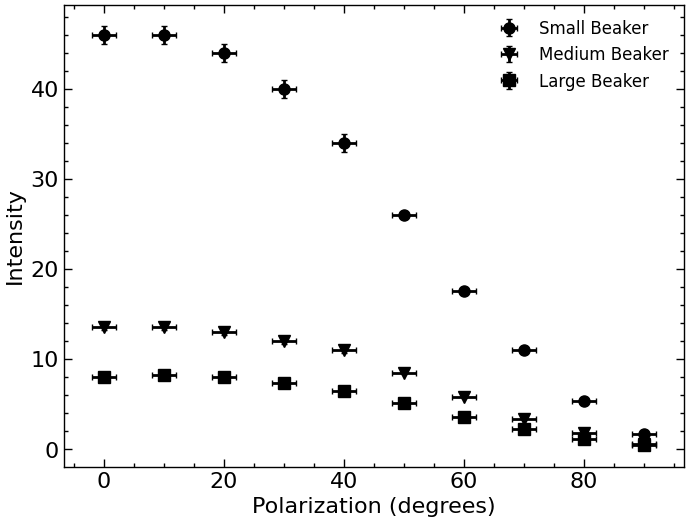
\includegraphics[width=\columnwidth]{../figures/solution3.png}
    \end{center}
    \caption{Intensity vs. Polarization for varying beaker sizes with solution 3. The polarization was measured in degrees and the intensity was measured in arbitrary units.}
    \label{solution3_figure}
\end{figure}

\begin{table}[H]
	\begin{center}
		\resizebox{\columnwidth}{!}{%
		\begin{tabular}{ccc}
			\toprule
			Polarization $\pm 2$ (degrees) & Intensity (arb. units) & Intensity $\pm$ (arb. units) \\
			\midrule
			\hline
			& Small Beaker & \\
			\hline
			90 & 1.20 & 0.03 \\
			80 & 3.8 & 0.1 \\
			70 & 9.2 & 0.1 \\
			60 & 16.0 & 0.3 \\
			50 & 24.5 & 0.3 \\
			40 & 32 & 1 \\
			30 & 38 & 1 \\
			20 & 43 & 1 \\
			10 & 46 & 1 \\
			0 & 46 & 1 \\
			\hline
			& Medium & \\
			\hline
			90 & 0.29 & 0.01 \\
			80 & 1.05 & 0.03 \\
			70 & 2.55 & 0.03 \\
			60 & 4.5 & 0.1 \\
			50 & 6.6 & 0.1 \\
			40 & 9.2 & 0.3 \\
			30 & 11.0 & 0.3 \\
			20 & 12.0 & 0.3 \\
			10 & 13.0 & 0.3 \\
			0 & 13.0 & 0.3 \\
			\hline
			& Large Beaker & \\
			\hline
			90 & 0.15 & 0.01 \\
			80 & 0.61 & 0.01 \\
			70 & 1.55 & 0.03 \\
			60 & 2.80 & 0.03 \\
			50 & 4.2 & 0.1 \\
			40 & 5.5 & 0.1 \\
			30 & 6.6 & 0.1 \\
			20 & 7.6 & 0.1 \\
			10 & 8.0 & 0.1 \\
			0 & 8.2 & 0.1 \\
			\bottomrule
		\end{tabular}}
	\end{center}
	\caption{Data for the small beaker, medium beaker, and large beaker with solution 4. The polarization was measured in degrees, and both intensity and intensity error were measured in arbitrary units.}
	\label{solution4_table}
\end{table}

\begin{figure}[H]
    \begin{center}
        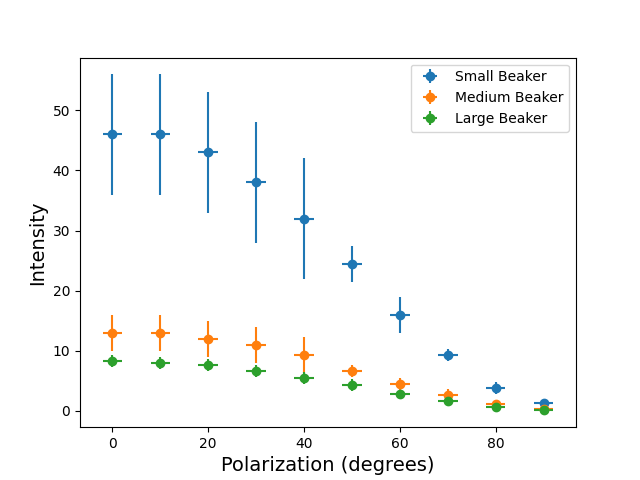
\includegraphics[width=\columnwidth]{../figures/solution4.png}
    \end{center}
    \caption{Intensity vs. Polarization for varying beaker sizes with solution 4. The polarization was measured in degrees and the intensity was measured in arbitrary units.}
    \label{solution4_figure}
\end{figure}

The following graph (\cref{solution4_small_beaker_fit_figure}) is an example of fitting a cosine function to the intensity versus polarization data for each concentration and beaker size. Fitting the data to this generic cosine function allowed us to extract the phase shift for each trial run.

\begin{figure}[H]
	\begin{center}
		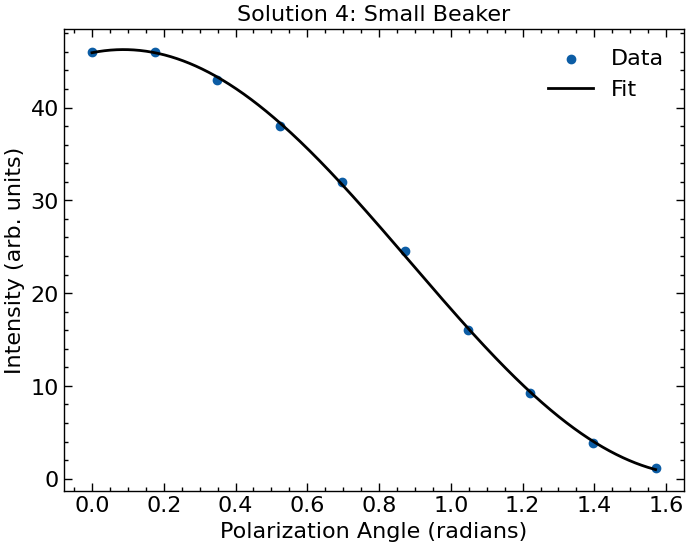
\includegraphics[width=\columnwidth]{../figures/solution4_small_beaker_fit.png}
	\end{center}
	\caption{Example graph of the intensity versus polarization angle plot for solution 4 in the small beaker to show how phase shift values were determined.}
	\label{solution4_small_beaker_fit_figure}
\end{figure}

\Cref{large_beaker_phase_shifts_figure,medium_beaker_phase_shifts_figure,small_beaker_phase_shifts_figure} show the phase shift as a function of sugar concentration in water, with each separate graph containing data from one beaker size. By representing phase shift versus sugar concentration, we can quantify how the polarization of light changes as a function of sugar concentration in water.

\begin{figure}[H]
    \begin{center}
        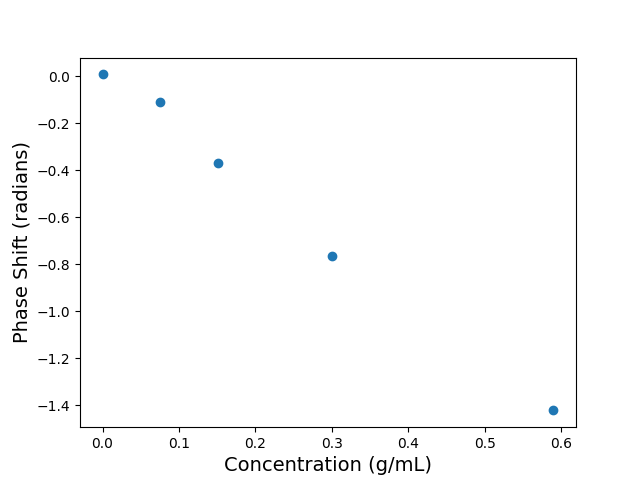
\includegraphics[width=\columnwidth]{../figures/large_beaker_phase_shifts.png}
    \end{center}
    \caption{Phase shift in radians versus concentration in grams per milliliter for the large beaker.}
    \label{large_beaker_phase_shifts_figure}
\end{figure}

\begin{figure}[H]
    \begin{center}
        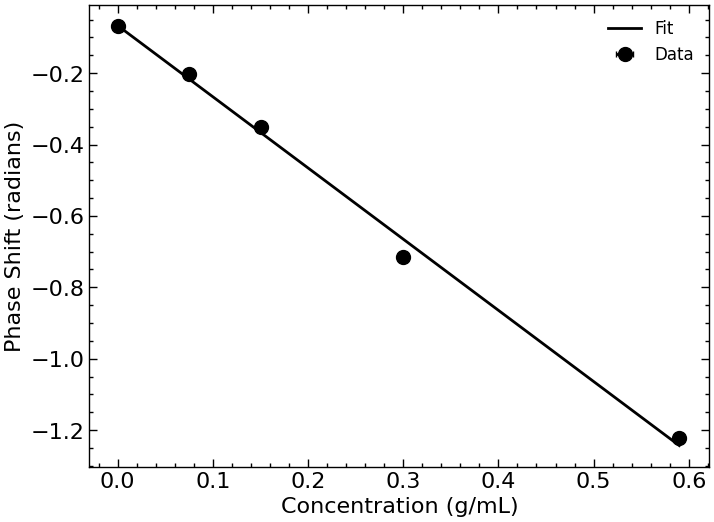
\includegraphics[width=\columnwidth]{../figures/medium_beaker_phase_shifts.png}
    \end{center}
    \caption{Phase shift in radians versus concentration in grams per milliliter for the medium beaker.}
    \label{medium_beaker_phase_shifts_figure}
\end{figure}

\begin{figure}[H]
    \begin{center}
        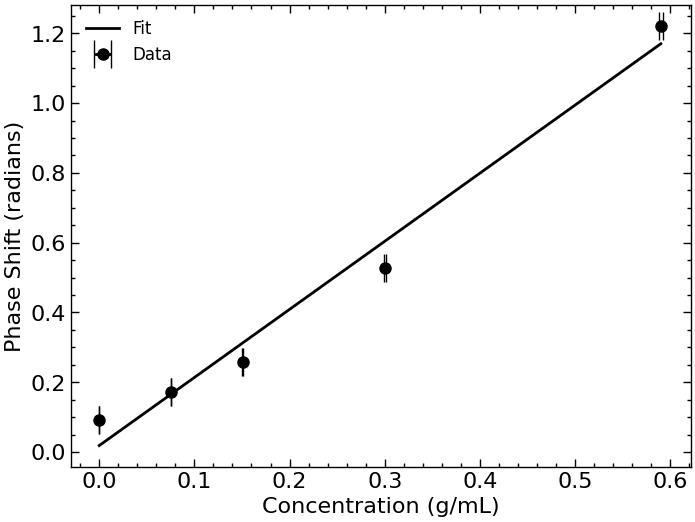
\includegraphics[width=\columnwidth]{../figures/small_beaker_phase_shifts.png}
    \end{center}
    \caption{Phase shift in radians versus concentration in grams per milliliter for the small beaker.}
    \label{small_beaker_phase_shifts_figure}
\end{figure}

\begin{figure}[H]
	\begin{center}
		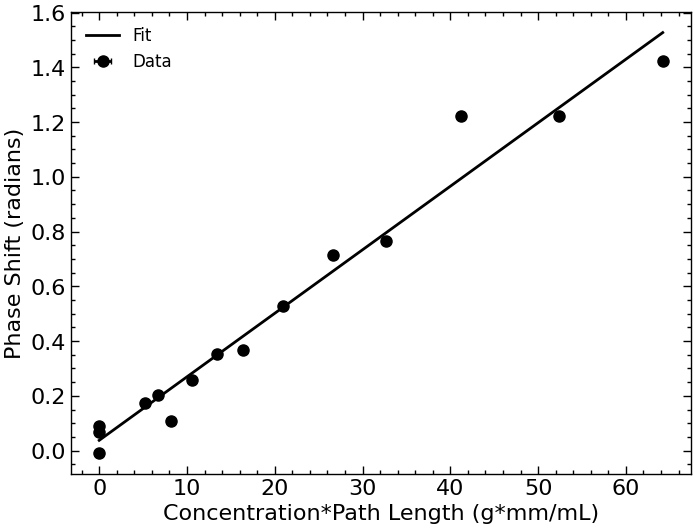
\includegraphics[width=\columnwidth]{../figures/concentration_times_diameter_phase_shifts.png}
	\end{center}
	\caption{This figure encapsulates the phase shift in radians as a function of both concentration in grams per milliliter and the path length in millimeters, where the horizontal axis is the product of the concentration and path length values.}
	\label{concentration_times_diameter_phase_shifts_figure}
\end{figure}

\begin{table}[H]
	\begin{center}
		\resizebox{\columnwidth}{!}{%
		\begin{tabular}{cccc}
			\toprule
			Solution \hspace{1mm} & Mass $\pm 0.1$ (g) \hspace{1mm} & Volume $\pm 2$ (mL) \hspace{1mm} & Concentration $\pm 0.001$ (g/mL) \\
			\midrule
			1 & 100.2 & 1000 & 0.100 \\
			2 & 200.2 & 1003 & 0.200 \\
			3 & 150.6 & 1000 & 0.150 \\
			4 & 75.3 & 1000 & 0.070 \\
			\bottomrule
		\end{tabular}}
	\end{center}
	\caption{Raw data for sugar solution concentrations with mass measured in grams, volume measured in mililiters, and concentration measured in grams per milileter.}
	\label{solution_concentration_table}
\end{table}

\begin{table}[H]
	\begin{center}
		\resizebox{5cm}{!}{%
		\begin{tabular}{cc}
			\toprule
			Beaker Label \hspace{2mm} & Beaker Diameter $\pm 0.1$ (mm) \\
			\midrule
			Small & 69.9 \\
			Medium & 88.8 \\
			Large & 108.8 \\
			\bottomrule
		\end{tabular}}
	\end{center}
	\caption{Raw data for the diameters (representing path length) of each beaker size in milimeters.}
	\label{beaker_diameters_table}
\end{table}